\documentclass[tikz,border=10pt,12pt,x11names]{standalone}
%%%<
\usepackage{verbatim}
%%%>
\usetikzlibrary{calc,arrows}
\usepackage{tikz}
\usepackage[]{circuitikz} % TiKZ Library for US Logic Circuits.
\usetikzlibrary{circuits.logic.US} % TiKZ Library for US Logic Circuits.
\usepackage{amsmath}

\usepackage{tikz}
\usetikzlibrary{circuits.logic.US} % TiKZ Library for US Logic Circuits.
\begin{document}
	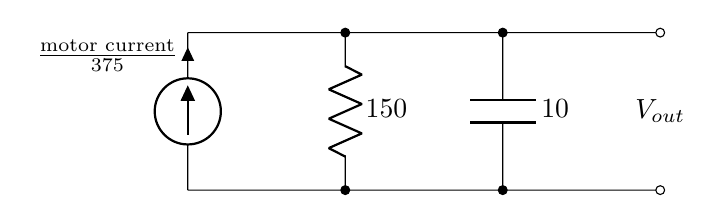
\begin{tikzpicture}[scale=2,american currents]
	
	
	\draw (0,0) to[I=$\frac{\textnormal{motor current}}{375}$] (0,1)
	(0,1) to[short,-o] (3,1)
	
	(1,1) to[R=150,*-*] (1,0)
	(0,0) to[short,-o] (3,0)
	
	(2,1) to[C=10 ,*-*] (2,0);
	
	
	\draw (3,0.5) node[]{$V_{out}$};
	
	\end{tikzpicture}
\end{document}